\chapter{Implementation}
\label{chap:implementation}

In this section, we outline the considerations taken into account and issues we had to work around while implementing. These come from a variety of sources, including the original implementation of \atwo{} and how Contiki works.

We begin by outlining the changes we have made to the \atwo{} protocol to accommodate the clustering implementation. We also explain some implementation specific details regarding the clustering and demote service and problems we had to solve.


\section{Modifications to \atwo{}}
The \atwo{} implementation has four layers as depicted in \cref{fig:a2-architecture}; our modifications compared to the original architecture in \cref{fig:original-a2-architecture} are underlined. The first layer, device drivers is not part of this thesis. However, we modified and added code to the other layers in order to implement clustering.

The cluster part of the Synchrotron layer handles several low-level details such as channel hopping, association, and modifications to the initiator. Also, we implement a clustering service which elects the CHs, announces them to the network, and lets every regular node select a cluster which it then joins using the join service from the \atwo{} layer. We also implement the demote service which runs after all clusters have run the join service, it demotes CHs that has fewer nodes than the parameter \emph{minimum cluster count}. Finally, we make some slight modifications to the application layer, to implement forwarding we change when a node is allowed to propose its value in an application.

\begin{figure}[bt]
    \centering
    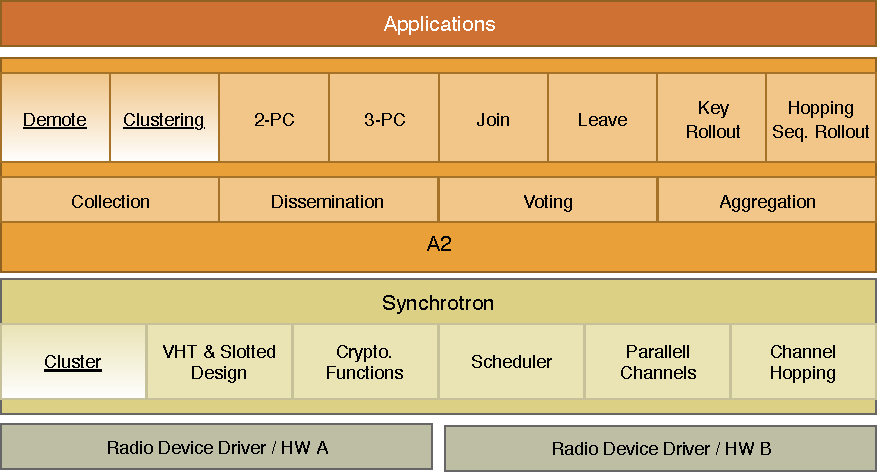
\includegraphics[width=0.7\textwidth]{figure/architecture.pdf}
    \caption{\textbf{Layered system architecture of \atwo{} \cite{a2-introduction-paper}.} Shows the placement of the cluster and demote modules in relation to the other modules. The Cluster module is required in Synchrotron to handle per-cluster channel hopping, association and scheduling modifications. The Clustering and demote services in \atwo{} contains the logic for electing and demoting cluster heads respectively.}
    \label{fig:a2-architecture}
\end{figure}

\subsection{Association}
%Before a node can communicate using the \atwo{} protocol, it has to associate with another node that is already a part of the network. In the beginning, the initiator starts the communication and acts as the source of truth for information regarding current round number, next application to be scheduled, and timing parameters for the communication among other things. When a node is trying to associate with the network, it listens for transmissions while occasionally hopping between random channels to maximise its chances to get a valid packet.

%Usually, all nodes will associate with the network when they start up, however, if a node does not receive a valid packet for some rounds or experiences a failure it will reassociate. The time, until all nodes have associated with the network (in rounds), is $\mathcal{O}(d)$, where $d$ is the diameter of the network. The reason for this time complexity is because a node shuts itself down until the next round as soon as it associates with the network.

With clustering implemented on \atwo{} we have to handle the fact that the network could already be partitioned into clusters when a node tries to associate with the network. If a node receives a packet from another node that is already in a cluster, and we are not currently in the process of clustering the network, the node joins that cluster. 

\subsection{Separating the Cluster Communication}
\label{subsec:separating-the-clusters}
We separate the clusters in two different ways. First, we use a modified version of the channel hopping in \atwo{}. The original \atwo{} implementation hops between radio channels in two different ways as outlined in \cref{subsec-frequency-agility}. Both a network wide predetermined sequence which all nodes follow to different channels and by using parallel channels, randomly selected from a small set. In our implementation, we separate the clusters into different channels. We deactivate the parallel channels functionality since one cluster should not be large enough to generate interference for itself. The nodes still follow the original hopping sequence but offset the channel number by the \textit{cluster-index}. The cluster-index is unique, deterministic and since it is an index the numbers are sequential which makes it ideal to use for this purpose.

Second, each node includes its cluster id in the packet header; if a node receives a packet from another cluster, the node discards that packet. During CH rounds they do not check this condition since all nodes are acting as forwarders. Moreover, during CH rounds, the constructive interference used by \atwo{} in the completion phase does not work. It does not work because CHs include their cluster id in all packets they send, which means that the packets in the completion phase are not equal. A possible solution could be to set the cluster id to 0 during CH rounds. Cluster ids are not used in the inter-cluster communication. However, if a node tries to associate with a packet containing no cluster id, it will not be able to join a cluster and therefore go back to associating. Due to time constraints we have not explored any other possible solutions for this problem.

\subsection{Forwarders During Cluster Head Rounds}
Since the HEED algorithm aims to assign non-overlapping cluster-heads, the communication between the cluster heads requires assistance to function. Therefore, during CH-rounds all non-CH nodes act as forwarders. We implement the forwarders by letting all nodes run the max application as usual but with the modification that nodes suggest 0 as their maximum value which is always overwritten by the CHs actual max value.

A more general implementation is possible since forwarders do not propose any new information by themselves they only require the knowledge of how to merge two packets for an application. We did, however, not implement such a solution since the \atwo{} model does not let the applications provide an operator for combining two payloads. If applications would provide that merge operation through an interface, then a more general implementation in \atwo{} could use the current running applications knowledge of how to merge packets without actually running the application. 


\subsection{Flags Field for Cluster Heads}
To separate CH rounds from cluster rounds, the nodes switch back and forth between intra- and inter-cluster communication every other round. However, during the join service, no CH rounds are executed. The reason for this is that while the join service's purpose is to build the flags field used for completion during communication within the clusters, the CH has their join process during the cluster service. Therefore, the CH already knows how they perform completion when the join service starts. More specifically, during the clustering service, the CHs builds a list of all CHs. Each CH then uses the index of their entry in this list as their index in the flags field. This both ensures that the CHs has sequential indexing of the flags field, and also know the length of the flags field. During CH rounds the CHs still use the same procedure as during cluster rounds; however, their index in the flags field corresponds to their index in the CH list built during the clustering service.

\subsection{The Initiator}
\label{subsec:implementation_the-initiator}
In our implementation, there are three different phases of the protocol, and the initiator is different in each of them. First, when either the clustering service or the demote service is running, the network is using a single preconfigured node as the initiator. Second, during cluster rounds each CH acts as the initiator in their cluster; since each cluster communicates on separate channels and every initiator runs synchronously with the other CHs, this does not create any conflicts in the network. Third, during CH rounds, to avoid having more than one initiator in the network the first CH in the CH list initiates the network communication.

Switching the initiator between different nodes introduce problems which we did not foresee. Namely, the network can end up in a state where no node consider themselves initiator and the network spends the rest of the time associating. What happens is one of two cases. Either, the preconfigured initiator node loses connection with the network during a round where it does not consider itself initiator and does not regain the connection before the network collectively switches to use that node as initiator again. Alternatively, the CH that is initiator during CH rounds loses connection to the network and demotes itself, the network cannot handle this case, and there will be no initiator during CH rounds until the network executes the clustering service again. 

We can mitigate both of these cases using a number of solutions. We briefly discuss two of them here together with their strengths and weaknesses. First, always using the preconfigured initiator regardless of the state of the network would completely solve this problem. However, this would create an even higher dependency on this node, increasing its energy usage potentially reducing the lifetime of that node and therefore the network. Furthermore, we would have to handle the cluster the preconfigured node joins as a special case to avoid having two initiators in that cluster. Second, we could use a fallback error handling scheme. If the preconfigured initiator is stuck associating it could assign itself as initiator again due to one of two triggers. First, it could use a timeout of some number of rounds; if it does not receive any packet before the timeout triggers, it assumes that the whole network is stuck associating and needs someone to be the initiator. Second, if its estimated time reaches a round in which it should be the initiator, for instance, when the clustering service should be running, it just starts broadcasting as the initiator, assuming the rest of the network will follow. This solution is, however, not very reliable. It assumes that the initiator node can keep correct time synchronisation without any external input, if its clock drifts too much it could wake up at the wrong time and start transmitting erroneous packets to the network. Nevertheless, this could prevent an unrecoverable standstill of the network.



\subsection{Interaction Between Services}
\label{subsec:interaction-between-services}
In this thesis, we implement two different services, the clustering service and the demote service. Furthermore, we use the join service provided by the \atwo{} protocol within the clusters to get consistency in the membership. However, for these applications to work properly, they have to be run in a specific order. First, the clustering service needs to be run and converge on a set of valid CHs. Following that, the network executes the join service within each cluster. Then the demote service is executed, by running the join service before the demote service each CH know how many nodes joined their cluster and can, therefore, make the decision to demote themselves or not. When the demote service is done, the join service needs to be rerun, since the clusters might have changed the network needs to make sure that any node that changed cluster is correctly picked up by that cluster. At this point the clustering process is complete, and operation of the network can resume as normal.




\section{The Clustering Service}
In this section, we explain some implementation specific details that are related to the clustering service. We go into detail about the packet payload, what information we transmit from a node and why; we also talk about issues we face due to not having completion flags. Finally, we talk about the catch-up mechanism we implemented in the clustering service to handle nodes joining the clustering process late.

\subsection{The Cluster Service Packet Payload}
As mentioned in the design chapter, the clustering service exchanges much information to inform the network of how many cluster heads have announced themselves. In this section, we describe the packet's content, why we include that information in the payload and the limitations we encountered when using this structure in the payload.

The cluster service payload contains information both about the cluster heads the transmitting node knows about and information about that node. The content of the cluster service packet payload is summarised in \cref{table:cluster-service-packet}. The cluster head list contains all the cluster heads the transmitting node knows about. The list contains information about the ID; the hop count; and the status of each cluster head, which is either \emph{Tentative} or \emph{Final}. The cluster head list uses three bytes of space per entry in the list with a maximum of 90 bytes allowing 30 entries. The transmitting node also includes its ID in the packet; this information is used in the clustering service to approximate the distance to other nodes as well as how dense the network is. The last entry is consecutive cluster rounds which is a counter that contains information about how many rounds has elapsed since the clustering service started to run; we use this parameter in the catch-up mechanism which we explain in \cref{subsec:catch-up-mechanism}. 

The packet payload size is restricted by the maximum packet size for the IEEE 802.15.4 standard, which is 127 bytes \cite{IEEE-802-15-4}. It is restricted further by the \atwo{} header size and some link layer data, giving us a maximum of 112 bytes for the payload size. As can be seen in \cref{table:cluster-service-packet}. We leave 22 bytes of space in the packet for two reasons. First, some features which we are not using in \atwo{} take up space in the packet header, we do not want the clustering service to break when other unrelated features are used. Second, by leaving some space, we allow more information to be added at a later date if someone should so decide.

\subsection{Clustering Without Completion Flags}
There are two problems introduced by the fact that we cannot run the consistent group membership protocol (the join service) before the clustering service. The problems are both caused by the restriction of the packet size. These two problems impose a hard limit on the number of CHs that can announce themselves in the network as well as increase the amount network of communication that occurs in the clustering service.

The first problem is that the clustering service does not have any flags field it can use to keep track of which nodes have learnt of which clusters. Using such a field would impose a limit on the total number of nodes the protocol can handle, and it would directly contradict one of the primary goals of this thesis, namely scaling. However, without the flags field, we cannot perform completion flooding or early turnoff, two prominent features of the Chaos protocol \cite{chaos-introduction-paper}. However, it is vital that all nodes learn of all CHs since they use this list as a substitute for the join service when running CH rounds. To increase the likelihood of the cluster head list being consistent across all nodes we store the packet payload in two different variables, one that represents the current knowledge of the network and one that represents this specific nodes knowledge. The first variable is reset at the beginning of every round forcing all CHs to transmit their status as CH again while the second variable is stored between rounds so that a node cannot forget anything it has learned so far.  By forcing the network to agree on a set of CH every round we increase the amount of network communication and thus the chance that any particular node will learn of the CHs that have announced themselves.

The size of the CH list in the packet payload causes the second problem. Since we use the list to substitute indices assigned by the join service, it has to be consistent across all nodes, which means that we can never have more CHs in the network than the maximum size of this list. It is not possible to discard CHs that, for example, are outside of a nodes competition radius since then some parts of the network would not consider that CH when calculating their completeness.

These two problems are a limitation on our implementation. It should be entirely possible to modify the consistent group membership protocol so that it can not only run for each cluster but also for the cluster heads eliminating the need for the clustering service to be consistent in that regard. Nodes could then filter out the CHs that are outside of their competition radius since no nodes should join a CH outside that parameter value. However, due to time limitations, we have not explored this implementation any further.




\begin{table}[bt]
\centering
\caption{The parameters and their sizes in the cluster service packet payload.}
\label{table:cluster-service-packet}
\begin{tabular}{|l|l|}
\hline
\textbf{Name}               & \textbf{Size(bytes)} \\ \hline
Cluster head count          & $1$                    \\
Source ID                   & $1$                    \\
Received packets count      & $24$                    \\
Cluster head list           & $3*30=90$              \\
Consecutive cluster rounds  & $1$                    \\ \hline
\textbf{Total}              & \textbf{95}          \\ \hline
\end{tabular}
\end{table}

\subsection{The Catch-up Mechanism}
\label{subsec:catch-up-mechanism}
By the definition of the HEED protocol, every node doubles the probability to announce themselves as tentative cluster heads each round. However, there is a problem if a node associates with the network during the execution of the clustering service. Specifically, its probability to announce itself as CH, $CH_{prob}$, will have fallen behind compared to other nodes; this is most noticeable in the early rounds of the network during the initial association of all nodes. For example, nodes associating with the initiator in round one randomises their initial $CH_{prob}$ in round two. However, in round two the initiator has already doubled its own $CH_{prob}$. As a remedy, we implemented a \textit{catch-up mechanism}. In the cluster service's packet payload, we attach a counter for the number of consecutive cluster rounds which a node saves once received. At the beginning of later rounds, they increment the counter before transmitting it on. The counter describes the number of times each node's initial $CH_{prob}$ should have doubled since the start of the clustering service. An advantage remains for nodes already part of the network or the ones which join earlier in the service, since they have had more chances to announce themselves as CH. However, as \cref{tab:prob-no-catchup} and \cref{tab:prob-catchup} show this advantage is very small.

\begin{table}[bt]
\centering
\caption{Probability that a node has announced itself as CH at a specific round without the catch-up mechanism.}
\label{tab:prob-no-catchup}
\begin{tabular}{|c|c|c|cccccc|}
\hline
\textbf{Round(r)} & \textbf{$CH_{Prob}$} & \multicolumn{7}{c|}{\textbf{Cumulative probability starting at round r}}                                                                                       \\ \hline
1                 & 0.005                & 0.005 &                            &                            &                            &                            &                            &       \\ \cline{1-4}
2                 & 0.010                & 0.015 & \multicolumn{1}{c|}{0.005} &                            &                            &                            &                            &       \\ \cline{1-5}
3                 & 0.020                & 0.035 & \multicolumn{1}{c|}{0.015} & \multicolumn{1}{c|}{0.005} &                            &                            &                            &       \\ \cline{1-6}
4                 & 0.040                & 0.073 & \multicolumn{1}{c|}{0.035} & \multicolumn{1}{c|}{0.015} & \multicolumn{1}{c|}{0.005} &                            &                            &       \\ \cline{1-7}
5                 & 0.080                & 0.147 & \multicolumn{1}{c|}{0.73}  & \multicolumn{1}{c|}{0.035} & \multicolumn{1}{c|}{0.015} & \multicolumn{1}{c|}{0.005} &                            &       \\ \cline{1-8}
6                 & 0.160                & 0.284 & \multicolumn{1}{c|}{0.147} & \multicolumn{1}{c|}{0.073} & \multicolumn{1}{c|}{0.035} & \multicolumn{1}{c|}{0.015} & \multicolumn{1}{c|}{0.005} &       \\ \hline
\textbf{7}                 & \textbf{0.320}                & \textbf{0.513} & \multicolumn{1}{c|}{\textbf{0.284}} & \multicolumn{1}{c|}{\textbf{0.147}} & \multicolumn{1}{c|}{\textbf{0.073}} & \multicolumn{1}{c|}{\textbf{0.035}} & \multicolumn{1}{c|}{\textbf{0.015}} & \textbf{0.005} \\ \hline
\end{tabular}
\end{table}

    
\begin{table}[bt]
\centering
\caption{Probability that a node has announced itself as CH at a specific round with the catch-up mechanism.}
\label{tab:prob-catchup}
\begin{tabular}{|c|c|c|cccccc|}
\hline
\textbf{Round(r)} & \textbf{$CH_{Prob}$} & \multicolumn{7}{c|}{\textbf{Cumulative probability starting at round r}}                                                                                       \\ \hline
1                 & 0.005                & 0.005 &                            &                            &                            &                            &                            &       \\ \cline{1-4}
2                 & 0.010                & 0.015 & \multicolumn{1}{c|}{0.010} &                            &                            &                            &                            &       \\ \cline{1-5}
3                 & 0.020                & 0.035 & \multicolumn{1}{c|}{0.030} & \multicolumn{1}{c|}{0.020} &                            &                            &                            &       \\ \cline{1-6}
4                 & 0.040                & 0.073 & \multicolumn{1}{c|}{0.069} & \multicolumn{1}{c|}{0.060} & \multicolumn{1}{c|}{0.040} &                            &                            &       \\ \cline{1-7}
5                 & 0.080                & 0.147 & \multicolumn{1}{c|}{0.143} & \multicolumn{1}{c|}{0.134} & \multicolumn{1}{c|}{0.117} & \multicolumn{1}{c|}{0.080} &                            &       \\ \cline{1-8}
6                 & 0.160                & 0.284 & \multicolumn{1}{c|}{0.280} & \multicolumn{1}{c|}{0.273} & \multicolumn{1}{c|}{0.258} & \multicolumn{1}{c|}{0.227} & \multicolumn{1}{c|}{0.160} &       \\ \hline
\textbf{7}                 & \textbf{0.320}                & \textbf{0.513} & \multicolumn{1}{c|}{\textbf{0.511}} & \multicolumn{1}{c|}{\textbf{0.506}} & \multicolumn{1}{c|}{\textbf{0.496}} & \multicolumn{1}{c|}{\textbf{0.474}} & \multicolumn{1}{c|}{\textbf{0.429}} & \textbf{0.320} \\ \hline
\end{tabular}
\end{table}


To motivate the advantage of having the catch-up mechanism we present the probability that a node has announced itself as CH after round $r$ without the catch-up mechanism in \cref{tab:prob-no-catchup} and with the catch-up mechanism in \cref{tab:prob-catchup}. The current starting probability of a node with maximum energy in our implementation is $CH_{prob} = 0.005$. Since the probability for a node to announce itself as CH is independent in each round, we can calculate the probability of a node having announced itself in the first $r$ rounds using the formula:

\begin{equation}
1 - \prod_0^r (1 - 2^rCH_{Prob}).   
\end{equation}

Looking at \cref{tab:prob-no-catchup} and \cref{tab:prob-catchup} the most interesting data points are the two bottom rows, emphasised in bold. Without the catch-up mechanism, there is a significant difference in the cumulative probability that a node has announced itself as CH. However, with the catch-up mechanism, the difference is minimal except for in the most extreme case when a node starts at round seven, compared to a node that started at round one. A specific example shows that when we do not use the catch-up mechanism a node that starts the clustering service at round three will at round seven have a $0.513 - 0.147 \approx 38$ percentage points less chance of having announced themselves as CH compared to a node that started at round one. However, with the catch-up mechanism the difference is only $0.513 - 0.506 \approx 0.7$ percentage points. The same pattern can be seen for other starting points as well, giving a clear motivation that the catch-up mechanism is useful. 

Another solution, which on the surface would seem to be fairer, would be to calculate the cumulative probability that a node should have announced itself if they would have been present from the beginning. Try to announce itself once using that probability, and then continue with the usual probabilities. However, consider a node which starts the clustering service together with the initiator, fails a couple of rounds later and then associates with the initiator again continuing with the clustering service. If we implement this solution, then a node that performed this sequence of events would have an advantage compared to nodes that did not fail. The advantage could be taken into consideration and excluded, but we chose the catch-up mechanism for its simplicity compared to the solution just described.





\subsection{The Demote Service}
The demote service is responsible for removing CHs that are considered suboptimal. It demotes all CHs which have fewer nodes in their cluster than the parameter \emph{minimum cluster size}. As we mention in \cref{subsec:interaction-between-services}, the join service is required to run before and after the demote service to ensure both that the demote service knows which CHs to demote and also for the user application to behave correctly.

The demote service behaves similarly to the clustering service; each CH decides to demote itself locally. The service is then run for some number of rounds to ensure that the information spreads to the whole network. At the end of the last demote service round each demoted CH, and all nodes that joined them select a new CH from the list of CHs that remain. Additionally, all nodes update their cluster indices according to the new list after they have removed all demoted CHs from the CH list.
